\documentclass[10pt,a4paper]{article}
\usepackage[margin=2.2cm]{geometry}
\usepackage{amsmath,amssymb,amsthm}
\usepackage{booktabs,graphicx,caption}
\usepackage{xurl}
\usepackage[hidelinks]{hyperref}
\usepackage{microtype}

\newtheorem{proposition}{Proposition}
\newtheorem{corollary}{Corollary}
\theoremstyle{definition}
\newtheorem{definition}{Definition}
\theoremstyle{remark}
\newtheorem{remark}{Remark}

\makeatletter\let\inputtable\@@input\makeatother
\newcommand{\E}{\mathbb{E}}
\newcommand{\Var}{\operatorname{Var}}

\title{The Sharma Absolute Boundary Summation (ABS) Model:\\
A Bounded, Sign-Preserving Multiplicative Noise Factor\\ for Embedded Simulation}
\author{Nitish Sharma\\
\small Embedded Software Engineer \& Independent Researcher\\
\small \texttt{nitish.ns378@gmail.com}}
\date{October 2026 (revised)\thanks{This version supersedes the draft of February 2026.
The quantization result reported there (the ``Magic~11'' effect) was an artifact of
histogram binning; it is corrected in Section~\ref{sec:distinct}. The statistical table of
the earlier draft is replaced by exact values with stated parameters.}}

\begin{document}
\maketitle

\begin{abstract}
We study the Sharma Absolute Boundary Summation (ABS) model, a multiplicative noise factor
$\eta = N/(N+S)$, where $S$ is a sum of $n$ independent uniform integers on $[a,b]$ and
$N=n(|a|+|b|)$. The factor is applied to a deterministic signal as
$v = v_{\text{ideal}}\,[1+\alpha(\eta-1)]$. We prove that the denominator can never vanish
when $b\neq 0$, that $\eta$ is strictly positive and bounded (in $[2/3,2]$ for symmetric
bounds), and that the multiplier preserves the sign of the signal for $0\le\alpha\le1$.
We give the exact distribution of $\eta$ as a finite sum, closed-form approximations of
its mean and variance, and show that $\eta$ is the reciprocal transform of a scaled
Irwin--Hall variate. A practical consequence is that the noise amplitude is set by $n$ and
$\alpha$, and is almost independent of the bounds $[a,b]$, which only set the quantization.
$\eta$ has a positive bias, $\E[\eta]>1$, which we quantify and remove by an exact
normalization. Shifting the bounds away from zero controls the skew, from about $+0.9$ down
to nearly symmetric. We use these properties to build a datasheet-calibrated sensor model
whose simulated readings never exceed the manufacturer's accuracy limit; Gaussian noise with
the same spread exceeds it on up to $0.9\%$ of readings in a stress test. Compared with other
bounded generators, ABS is not the most flexible (Beta distributions cover more shapes), but
it is the only one in our comparison that is integer-only, constant-time and skew-adjustable,
at about one fifth of the cost of Beta-distributed noise on our test host. We provide
floating-point and integer-only (Q16.16) implementations and reproducible experiments, and
state the model's limitations: it produces white, thin-tailed noise, and it does not replace
coherent noise or heavy-tailed financial models.
\end{abstract}

\section{Introduction}
Testing embedded firmware and simulations often requires perturbing a deterministic
signal (a sensor reading, a velocity, a timing value) with noise whose size scales with the
signal. Multiplicative noise of the form $v=v_{\text{ideal}}(1+\epsilon)$ is the standard
choice for this \cite{gardiner,kloeden}. When $\epsilon$ is Gaussian, generating it needs
either transcendental functions (Box--Muller \cite{boxmuller}) or a sum of uniforms
(the Irwin--Hall approximation \cite{irwin,hall}), and the factor $1+\epsilon$ can become
zero or negative, which flips the sign of the signal.

The ABS model builds the factor from a bounded integer sum and a single division. This
paper makes the following contributions:
\begin{enumerate}
\item proofs that the factor is always defined, strictly positive and bounded, and that the
perturbed signal keeps its sign (Section~\ref{sec:props});
\item the exact distribution of $\eta$, closed-form moments, and its relation to the
Irwin--Hall distribution (Sections~\ref{sec:dist}--\ref{sec:ih});
\item design rules for $n$ and $\alpha$, and an exact bias correction
(Section~\ref{sec:design});
\item float and integer-only implementations with an unbiased integer sampler, and
reproducible experiments (Sections~\ref{sec:impl}--\ref{sec:exp});
\item skew control through the bounds, and a datasheet-calibrated sensor model that never
exceeds the stated accuracy limit (Sections~\ref{sec:ih} and \ref{sec:sensor});
\item a comparison with other bounded generators on cost, determinism and attainable shapes
(Section~\ref{sec:compare}).
\end{enumerate}
We aim for a small, well-characterized engineering tool, and we state where it should not be
used (Section~\ref{sec:limits}).

\section{Definition}
\begin{definition}[Sharma ABS factor]
Let $a<b$ be integers, $n\ge1$, and $r_1,\dots,r_n$ independent and uniform on
$\{a,a+1,\dots,b\}$. Define
\begin{equation}
W = |a|+|b|,\qquad N=nW,\qquad S=\sum_{i=1}^{n} r_i,\qquad
\eta=\frac{N}{N+S}.
\label{eq:eta}
\end{equation}
For an influence coefficient $\alpha\ge0$, the perturbed signal is
\begin{equation}
v_{\text{real}} = v_{\text{ideal}}\,\bigl[1+\alpha(\eta-1)\bigr]
= v_{\text{ideal}}\,\bigl[(1-\alpha)+\alpha\eta\bigr].
\label{eq:apply}
\end{equation}
\end{definition}
We call $n$ the \emph{complexity} and $[a,b]$ the \emph{bounds}. Throughout, $m=b-a+1$ is
the number of values each $r_i$ can take.

\section{Basic properties}\label{sec:props}

\begin{proposition}[No division by zero]\label{prop:denom}
For every outcome, $N+S\ge n(W+a)$. Moreover $W+a>0$ if and only if $b\neq0$. Hence the
denominator of \eqref{eq:eta} is strictly positive for every outcome if and only if $b\ne0$.
\end{proposition}
\begin{proof}
Each $r_i\ge a$, so $S\ge na$ and $N+S\ge n(W+a)$, with equality when all $r_i=a$, an
outcome of positive probability. If $a\ge0$ then $b>a\ge0$ and $W+a=2a+b>0$. If $a<0$ then
$W+a=|b|$, which is positive iff $b\ne0$.
\end{proof}

So the ``stability guard'' of the earlier draft (returning $1$ when the denominator is zero)
is only reachable when $b=0$. Implementations should reject $b=0$ instead.

\begin{corollary}[Bounds and positivity]\label{cor:bounds}
If $b\ne0$, $\eta$ is strictly positive and
\begin{equation}
\frac{W}{W+b}\;\le\;\eta\;\le\;\frac{W}{W+a}.
\end{equation}
For symmetric bounds $[-c,c]$, $c\ge1$, this is $2/3\le\eta\le2$ for every $c$ and $n$.
\end{corollary}
\begin{proof}
$\eta$ is decreasing in $S$, and $na\le S\le nb$; substitute both ends. Both ends are positive by
Proposition~\ref{prop:denom}.
\end{proof}

\begin{corollary}[Sign preservation]
If $b\ne0$ and $0\le\alpha\le1$, then $(1-\alpha)+\alpha\eta>0$, so $v_{\text{real}}$ has the
same sign as $v_{\text{ideal}}$, and $v_{\text{real}}=0$ only when $v_{\text{ideal}}=0$.
\end{corollary}

This is the precise version of the claim that ABS ``respects physical limits'': a
non-negative quantity (a voltage on a $0$--$5$\,V rail, a speed, a price) stays
non-negative. It does \emph{not} respect an upper limit: with $\alpha=1$ and symmetric
bounds, the signal can be multiplied by up to $2$ (Section~\ref{sec:limits}).

\section{Exact distribution}\label{sec:dist}

\begin{proposition}[States]\label{prop:states}
$\eta$ takes exactly $n(b-a)+1$ distinct values, one for each integer $s\in[na,nb]$, with
\begin{equation}
P\!\left(\eta=\tfrac{N}{N+s}\right)=P(S=s)
= m^{-n}\sum_{j\ge0}(-1)^j\binom{n}{j}\binom{k-jm+n-1}{n-1},\qquad k=s-na,
\label{eq:pmf}
\end{equation}
where binomials with negative upper index are zero. In $T$ independent draws, the expected
number of distinct values observed is
\begin{equation}
D(T)=\sum_{s=na}^{nb}\Bigl[1-\bigl(1-P(S=s)\bigr)^T\Bigr].
\label{eq:distinct}
\end{equation}
\end{proposition}
\begin{proof}
$S-na$ is a sum of $n$ independent uniforms on $\{0,\dots,m-1\}$; \eqref{eq:pmf} is the
standard inclusion--exclusion count of such compositions. The map $s\mapsto N/(N+s)$ is
strictly decreasing, so distinct sums give distinct $\eta$. Equation \eqref{eq:distinct}
follows from linearity of expectation over the indicator that state $s$ is seen.
\end{proof}

Because the support is finite, every moment of $\eta$ is a finite sum,
$\E[\eta^k]=\sum_s P(S=s)\,(N/(N+s))^k$, which can be evaluated exactly on a host computer
(in practice by convolving $n$ uniform PMFs). We use these exact values as ground truth.

\section{Moments, and the role of the bounds}\label{sec:ih}

Write $\eta=1/(1+X)$ with $X=S/N$. Then
\begin{equation}
\mu_X=\E[X]=\frac{a+b}{2W},\qquad
\sigma_X^2=\Var[X]=\frac{m^2-1}{12\,nW^2}.
\end{equation}
A second-order expansion of $1/(1+X)$ about $\mu_X$ (the delta method \cite{casella}) gives
\begin{equation}
\E[\eta]\approx 1-\mu_X+\mu_X^2+\sigma_X^2,\qquad
\operatorname{sd}(\eta)\approx\frac{\sigma_X}{(1+\mu_X)^2}.
\label{eq:approx}
\end{equation}

\paragraph{Symmetric bounds.} For $[a,b]=[-c,c]$, $\mu_X=0$ and
$\sigma_X^2=(c+1)/(12nc)$, so
\begin{equation}
\operatorname{sd}(\eta)\approx\sqrt{\frac{1+1/c}{12\,n}}\;\xrightarrow{c\to\infty}\;
\frac{1}{\sqrt{12n}},\qquad
\E[\eta]-1\approx\frac{1+1/c}{12\,n}>0.
\label{eq:sym}
\end{equation}
Two consequences follow. First, the noise amplitude is controlled by $n$, while $c$ only
matters through the factor $1+1/c$, which is between $1$ and $2$. Bounds of $[-10,10]$ and
$[-1000,1000]$ produce almost the same noise (Table~\ref{tab:moments},
Figure~\ref{fig:std}); larger bounds only make the quantization finer
(Proposition~\ref{prop:states}). Second, $\E[\eta]>1$. This is Jensen's inequality
\cite{jensen}: $x\mapsto1/(1+x)$ is strictly convex, so
$\E[\eta]>1/(1+\E[X])=1$ whenever $X$ is non-degenerate and $\E[X]=0$. With asymmetric
bounds the bias is larger because $\mu_X\ne0$; for $[-12,11]$, $\mu_X=-1/46$ and
$\E[\eta]=1.0305$.

\paragraph{Relation to Irwin--Hall.} As $c\to\infty$, $r_i/c$ tends to a continuous
uniform variable on $[-1,1]$, so $X\to(\sum_{i=1}^n U_i-n/2)/n$ with $U_i$ uniform on
$[0,1]$. Writing $Z_n$ for the standardized Irwin--Hall sum \cite{irwin,hall},
\begin{equation}
\eta\;\approx\;\frac{1}{1+Z_n/\sqrt{12n}} .
\end{equation}
For $n=12$ this is $1/(1+Z_{12}/12)$, where $Z_{12}=\sum U_i-6$ is the classical
``sum of twelve uniforms'' approximation to a standard normal variable \cite{knuth}. ABS is
therefore close to standard multiplicative near-Gaussian noise, $1-Z/\sqrt{12n}$, to first
order. The reciprocal adds a positive skew and keeps the factor positive and bounded, which
the plain Gaussian form does not.

\paragraph{The bounds set the skew.} Symmetric bounds leave the noise \emph{amplitude} almost
unchanged, but moving the bounds away from zero changes its \emph{shape}. With narrow positive
bounds, $X=S/N$ stays in a short interval around $\mu_X>0$ where $1/(1+X)$ is nearly linear,
so $\eta$ is nearly symmetric. Table~\ref{tab:skew} gives the exact skewness of $\eta$: from
about $+0.8$ for $[-10,10]$ down to $+0.03$ for $[900,1000]$. Negative skew is obtained by
mirroring, $2\E[\eta]-\eta$. A single integer generator therefore covers both symmetric and
right- or left-skewed bounded noise; we use this in Section~\ref{sec:sensor}.

\begin{table}[h]
\centering\small
\caption{Exact skewness of $\eta$ for several bounds.}
\label{tab:skew}
\begin{tabular}{lrrr}
\toprule
Bounds $[a,b]$ & $n=1$ & $n=4$ & $n=16$\\
\midrule
\inputtable tables/skew.tex
\bottomrule
\end{tabular}
\end{table}

\section{Design rules}\label{sec:design}

\paragraph{Amplitude.} By \eqref{eq:apply}, the multiplier $M=1+\alpha(\eta-1)$ has
$\operatorname{sd}(M)=\alpha\operatorname{sd}(\eta)$ and $\E|M-1|=\alpha\,\E|\eta-1|$:
every deviation statistic is \emph{exactly} linear in $\alpha$ (Table~\ref{tab:alpha}).
Since $n$ costs $n$ random draws per sample and $\alpha$ costs nothing, we recommend choosing
$n$ for the shape (larger $n$ means less skew and less bias) and then setting
\begin{equation}
\alpha=\frac{\sigma_{\text{target}}}{\operatorname{sd}(\eta)}\approx
\sigma_{\text{target}}\sqrt{\frac{12n}{1+1/c}} .
\end{equation}
For example, $\sigma_{\text{target}}=2\%$ with $n=12$, $c=10$ gives $\alpha\approx0.22$.
Keeping $\alpha\le1$ preserves the sign guarantee; this limits the amplitude to
$\operatorname{sd}(\eta)$.

\paragraph{Bias correction.} If a mean multiplier of exactly one matters, use
$\tilde\eta=\eta/\E[\eta]$ with $\E[\eta]$ computed exactly once on the host (Section~\ref{sec:dist}).
Then $\E[\tilde\eta]=1$, $\E[M]=1$, and positivity is unchanged. For $[-10,10]$, $n=12$, the
constant is $1.0078$.

\paragraph{Bounds.} For amplitude, symmetric bounds $[-c,c]$ with $c$ chosen only for
resolution: the factor has $2nc+1$ levels, which matters only for very small $c$
(e.g.\ $c=1$, $n=12$ gives 25 levels). For shape, shift the bounds
(Table~\ref{tab:skew}): narrow positive bounds such as $[900,1000]$ give nearly symmetric
noise, bounds around zero give right-skewed noise.

\section{Implementation}\label{sec:impl}
The reference C implementation is a single header with no dependencies beyond
\texttt{stdint.h}. It uses:
\begin{itemize}
\item a seeded xorshift32 generator \cite{marsaglia}, with a re-entrant variant that takes
the state as an argument (for ISRs and threads);
\item Lemire's multiply-shift method with rejection \cite{lemire} to draw unbiased integers
on $[a,b]$. The earlier \texttt{rand() \% m} has modulo bias and was never seeded. A redraw
happens with probability below $m/2^{32}$ per value; where strictly constant time is required,
the rejection step can be dropped at a bias of the same negligible size;
\item an integer-only path that returns $\eta$ in Q16.16 format. When $N<2^{16}$ it needs one
32-bit unsigned division, which is a single instruction on Cortex-M3/M4/M7. Otherwise it
falls back to a 64-bit division;
\item input validation that rejects $n\le0$ and $b=0$ (Proposition~\ref{prop:denom}).
\end{itemize}
With $|a|,|b|,n\le 2^{15}-1$ every intermediate fits in a signed 32-bit integer. On our
test host the Q16 result differs from the float result by at most one Q16 step
($1.5\times10^{-5}$) over $2\times10^6$ draws.

\section{Experiments}\label{sec:exp}
All numbers below are produced by \texttt{analysis/make\_paper\_results.py} (seed 2026) and
\texttt{analysis/bench.c} in the repository.

\subsection{Moments: exact, approximate and simulated}
Table~\ref{tab:moments} compares exact moments from \eqref{eq:pmf}, the approximations
\eqref{eq:approx}, and $10^6$ Monte Carlo draws. The exact and simulated values agree to
within sampling error. The approximation of the mean is within $0.002$, and the
approximation of the standard deviation is within $9\%$ for small $n$ and within $1\%$ for
$n\ge48$.

\begin{table}[h]
\centering\small
\caption{Moments of $\eta$. ``Ex.''\ exact, ``Appr.''\ Eq.~\eqref{eq:approx}, ``MC''\ $10^6$ draws.}
\label{tab:moments}
\begin{tabular}{lrrrrrrrrr}
\toprule
& & & \multicolumn{3}{c}{$\E[\eta]$} & \multicolumn{3}{c}{sd$(\eta)$} & skew\\
\cmidrule(lr){4-6}\cmidrule(lr){7-9}
Bounds & $n$ & states & Ex. & Appr. & MC & Ex. & Appr. & MC & Ex.\\
\midrule
\inputtable tables/moments.tex 
\bottomrule
\end{tabular}
\end{table}

\begin{figure}[h]
\centering
\begin{minipage}{0.48\linewidth}\centering
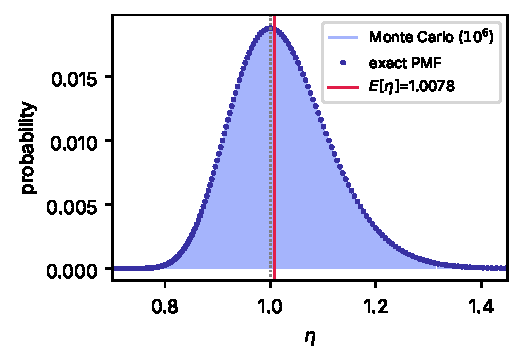
\includegraphics[width=\linewidth]{figs/pmf.pdf}
\caption{Exact distribution of $\eta$ for $[-10,10]$, $n=12$, against $10^6$ draws. The
distribution is right-skewed and its mean exceeds 1.}
\label{fig:pmf}
\end{minipage}\hfill
\begin{minipage}{0.48\linewidth}\centering
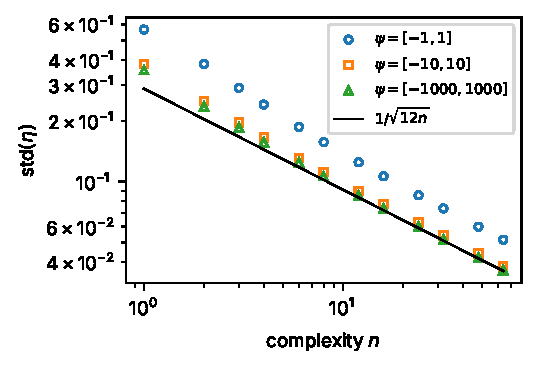
\includegraphics[width=\linewidth]{figs/std_vs_n.pdf}
\caption{sd$(\eta)$ against $n$ for three bounds. The spread follows $1/\sqrt{12n}$ and
barely depends on the bounds.}
\label{fig:std}
\end{minipage}
\end{figure}

\subsection{Number of distinct values}\label{sec:distinct}
The earlier draft reported only 11 distinct values of $\eta$ in 100 trials for $n=12$,
$[-12,11]$, and 88 in 1000 trials for $n=50$, $[-50,50]$. Proposition~\ref{prop:states}
shows that this is not possible: these settings have 277 and 5001 states, and the expected
counts are about 61 and 566. Table~\ref{tab:distinct} confirms this over 20 independent
runs. The earlier figure of 11 most likely counted the occupied bins of a histogram of width
$0.02$ over $[0.9,1.1]$. There is no special bottleneck at $n=12$; the number of states is
always $n(b-a)+1$.

\begin{table}[h]
\centering\small
\caption{Distinct values of $\eta$: theoretical states, expected count $D(T)$ from
\eqref{eq:distinct}, and observed mean (range) over 20 runs.}
\label{tab:distinct}
\begin{tabular}{lrrrrl}
\toprule
Bounds & $n$ & $T$ & states & $D(T)$ & observed\\
\midrule
\inputtable tables/distinct.tex 
\bottomrule
\end{tabular}
\end{table}

\subsection{Effect of $\alpha$}
Table~\ref{tab:alpha} gives exact statistics of the multiplier $M$ for $[-10,10]$, $n=12$.
The mean absolute deviation and the $99.9\%$ two-sided deviation bound are exactly
proportional to $\alpha$. The mean of $M$ is $1+\alpha(\E[\eta]-1)$, which shows the bias
when no correction is applied.

\begin{table}[h]
\centering\small
\caption{Exact statistics of $M=1+\alpha(\eta-1)$, bounds $[-10,10]$, $n=12$, no bias correction.}
\label{tab:alpha}
\begin{tabular}{rrrr}
\toprule
$\alpha$ & $\E[M]$ & $\E|M-1|$ (\%) & 99.9\% bound on $|M-1|$ (\%)\\
\midrule
\inputtable tables/alpha.tex 
\bottomrule
\end{tabular}
\end{table}

\subsection{Cost}
Table~\ref{tab:bench} reports throughput on a desktop-class host (Intel Xeon at 2.1\,GHz,
GCC 13.3, \texttt{-O2}, $2\times10^7$ samples, median of 3 runs, the same xorshift32
generator for all methods). The cost of ABS is dominated by its $n$ random draws: it matches
Irwin--Hall with the same $n$, and it is slower than Box--Muller on a machine with a hardware
FPU and fast \texttt{libm}. The case for ABS on microcontrollers rests on its operation
count: integer additions and a single integer division, with no transcendental functions,
which are expensive on cores without an FPU. We have not yet measured cycle counts on
microcontroller targets; this is left for future work.

\begin{table}[h]
\centering\small
\caption{Host throughput (lower is faster). Not representative of microcontrollers.}
\label{tab:bench}
\begin{tabular}{llr}
\toprule
Method & Operations per sample & ns/sample\\
\midrule
\inputtable tables/bench.tex 
\bottomrule
\end{tabular}
\end{table}

\subsection{Illustrations}
Figure~\ref{fig:apps} applies the bias-corrected factor to two signals. On the left, a
sensor voltage between $0.1$ and $4.9$\,V is perturbed with $n=48$, $\alpha=0.5$. Near
$0$\,V the noise shrinks with the signal and the reading never goes negative. Near the top
of the range, however, the noisy signal exceeds the $5$\,V rail in 199 of 200
independent runs, and goes below $0$\,V in none. Users who need an upper limit must clip it explicitly. On the
right, a damped oscillation is perturbed with $n=12$; the noise decays with the envelope, as
expected from multiplicative noise.

\begin{figure}[h]
\centering
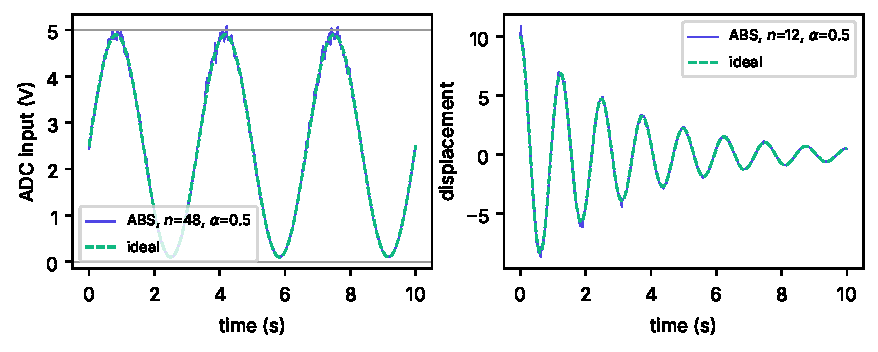
\includegraphics[width=0.9\linewidth]{figs/applications.pdf}
\caption{Left: ADC input on a $0$--$5$\,V rail; the lower rail is respected, the upper one
is not. Right: damped oscillation. Bias-corrected $\eta$ in both.}
\label{fig:apps}
\end{figure}

\section{Application: datasheet-calibrated sensor simulation}\label{sec:sensor}
Sensor datasheets state accuracy as a hard limit, for example ``$\pm$6\,cm up to 6\,m,
$\pm$1\% from 6 to 12\,m''. A simulated sensor should never report an error a compliant unit
cannot produce. Because $\eta$ is bounded, it can be turned into a \emph{unit error variable}
\begin{equation}
u=\frac{\eta-\E[\eta]}{D},\qquad D=\max\bigl(\eta_{\max}-\E[\eta],\ \E[\eta]-\eta_{\min}\bigr),
\end{equation}
with $\E[u]=0$ and $|u|\le1$ for every outcome. A reading of a true value $x$ is then
\begin{equation}
y=\operatorname{Q}\!\Bigl(x+|x|\,r\,[f g+(1-f)u_1]+e\,[f o+(1-f)u_2]\Bigr),
\label{eq:sensor}
\end{equation}
where $r$ and $e$ are the datasheet's relative and absolute accuracy (which may depend on
$x$), $g$ and $o$ are gain and offset errors drawn once per simulated unit, $u_1,u_2$ are
drawn per reading, $f\in[0,1]$ is the share of the error budget fixed per unit, and
$\operatorname{Q}$ rounds to the resolution and clips to the range. All four variables are unit
ABS draws.

\begin{proposition}[Datasheet compliance]
Every reading from \eqref{eq:sensor} satisfies $|y-x|\le r|x|+e+\delta/2$, where $\delta$ is
the resolution, for any realisation of the random draws.
\end{proposition}
\begin{proof}
$|fg+(1-f)u_1|\le f+(1-f)=1$ and likewise for the offset term, because $|g|,|o|,|u_1|,|u_2|\le1$.
Rounding adds at most $\delta/2$, and clipping to the range can only move the reading towards
$x$ when $x$ lies inside the range.
\end{proof}

The guarantee needs only boundedness, not ABS in particular (Section~\ref{sec:compare});
ABS contributes integer-only evaluation and the skew control of Table~\ref{tab:skew}.
Table~\ref{tab:presets} lists the presets in the code, with accuracy figures taken from the
manufacturers' documents \cite{tfmini,ds18b20,ina219}. Over 200 simulated units and
$2000$ readings each per preset, with $n=4$, the worst error was 60--81\% of the limit for
both shapes.

\begin{table}[h]
\centering\small
\caption{Sensor presets. Accuracy figures from the manufacturers' documents.}
\label{tab:presets}
\begin{tabular}{lll}
\toprule
Sensor & Accuracy & Resolution\\
\midrule
Benewake TFmini-S lidar \cite{tfmini} & $\pm$6\,cm (0.1--6\,m), $\pm$1\% (6--12\,m) & 1\,cm\\
DS18B20 thermometer \cite{ds18b20} & $\pm$0.5\,$^\circ$C ($-10$ to $+85\,^\circ$C) & 0.0625\,$^\circ$C\\
INA219B current, 0.1\,$\Omega$ shunt \cite{ina219} & 0.5\% gain + 100\,$\mu$V offset & --\\
\bottomrule
\end{tabular}
\end{table}

Figure~\ref{fig:sensor} stresses the TFmini-S model with $n=1$, so that errors come close to
the limit, and compares it with a model that has the same per-unit and per-reading spread but
Gaussian shape. Over 30 units $\times$ 400 readings, the ABS model reached 94\% of the limit and
never exceeded it; the Gaussian model exceeded it on 0.93\% of readings, by up to 45\%. Over
100 units $\times$ 2000 readings, the Gaussian out-of-spec rate was 0.92\% at $n=1$, 0.02\% at
$n=2$ and 0 at $n\ge4$; the ABS rate was 0 in every case. The difference therefore matters when
simulated noise is pushed towards the datasheet limit, which is exactly the regime of interest
for testing firmware tolerance checks.

\begin{figure}[h]
\centering
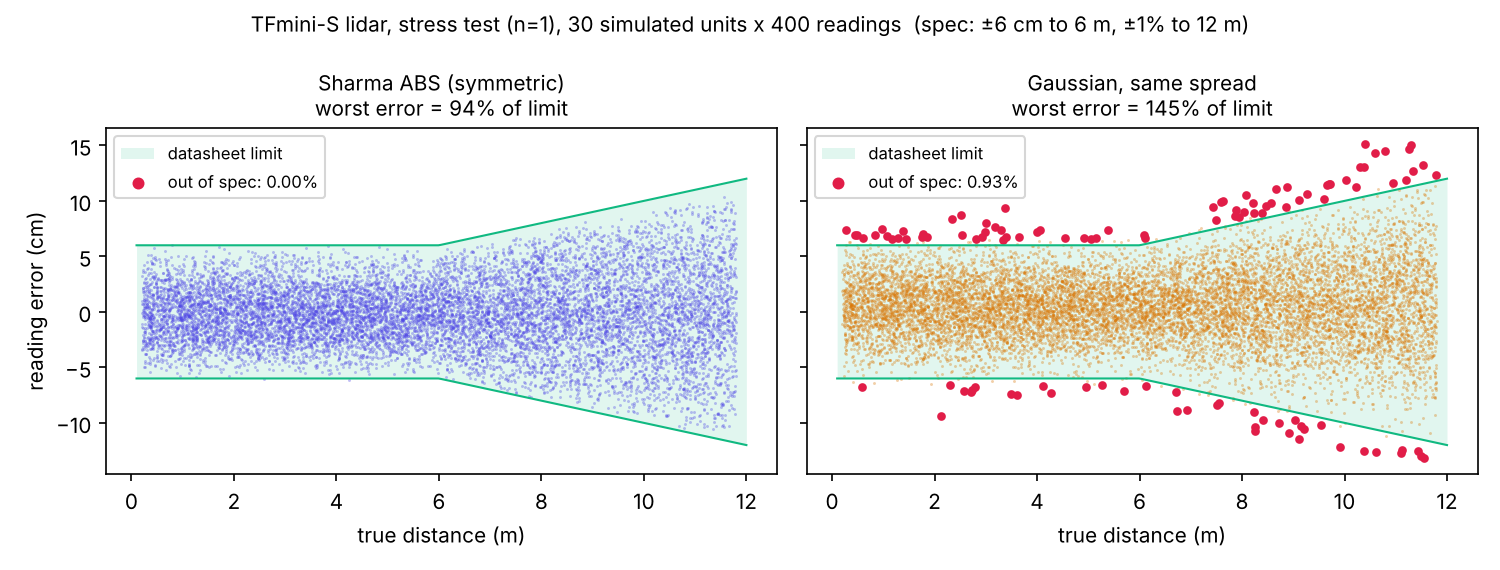
\includegraphics[width=0.95\linewidth]{figs/datasheet_sensor.png}
\caption{TFmini-S stress test ($n=1$): reading error against true distance for 30 simulated
units. Green band: datasheet limit. Red: readings outside it.}
\label{fig:sensor}
\end{figure}

\section{Comparison with other bounded generators}\label{sec:compare}
A reviewer may fairly ask why ABS should be used instead of a standard bounded distribution.
We compare it with Irwin--Hall sums \cite{irwin,hall}, clipped and truncated Gaussians,
Beta distributions (sampled from two gamma variates \cite{marsagliatsang}) and the triangular
distribution, all driven by the same xorshift32 generator.

\paragraph{Cost and determinism.} Table~\ref{tab:cost} gives host throughput (same setup as
Table~\ref{tab:bench}; range over two runs of three repetitions) together with the properties
that matter on microcontrollers: integer-only arithmetic, and a fixed amount of work per
sample, which bounds worst-case execution time. Truncated Gaussian and Beta samplers use
rejection loops; we observed up to 16 and 5 redraws respectively.

\begin{table}[h]
\centering\footnotesize
\caption{Bounded generators on the same RNG (host CPU, ns per sample). $^{*}$Apart from the
rare redraw in unbiased integer sampling (Section~\ref{sec:impl}).}
\label{tab:cost}
\begin{tabular}{p{3.4cm}lp{2.6cm}p{2.6cm}p{3.0cm}}
\toprule
Generator & ns/sample & Integer-only & Fixed work & Skew control\\
\midrule
\inputtable tables/cost.tex
\bottomrule
\end{tabular}
\end{table}

\paragraph{Attainable shapes.} Normalising every distribution to mean 0 and maximum $|u|=1$,
Figure~\ref{fig:coverage} and Table~\ref{tab:coverage} show which combinations of spread and
skew each family can produce. Beta distributions cover the widest region; truncated
Gaussians cover a broad central region; ABS covers skewness up to about $\pm1$ over a wide
range of spreads; Irwin--Hall is restricted to zero skew and the triangular family to a
narrow strip.

\begin{figure}[h]
\centering
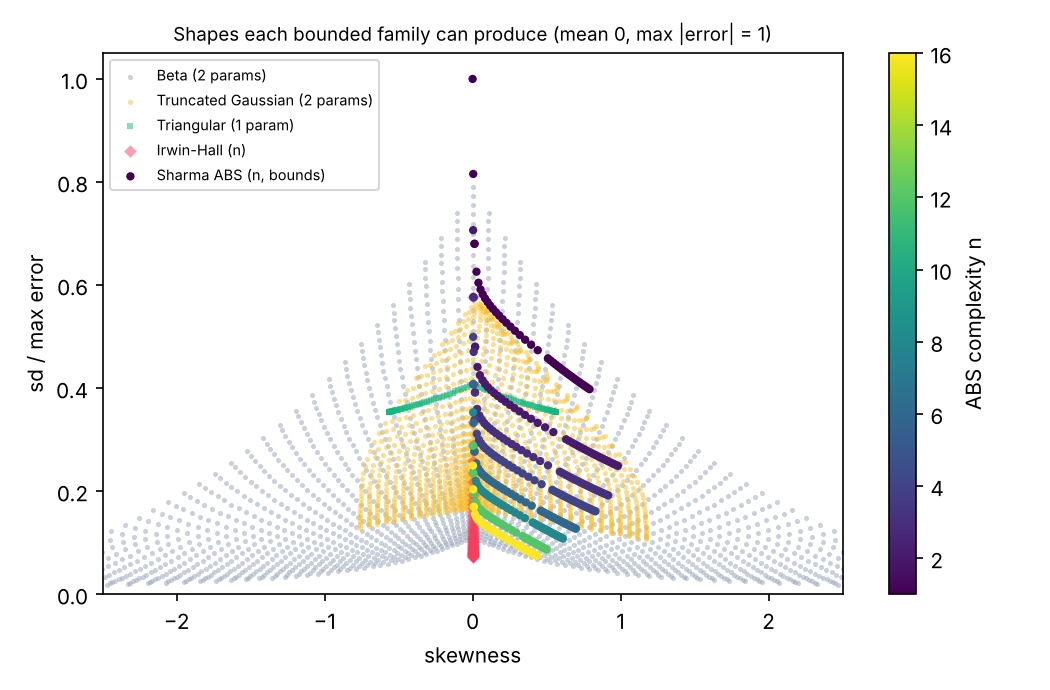
\includegraphics[width=0.75\linewidth]{figs/bounded_coverage.png}
\caption{Spread and skewness attainable by each bounded family (mean 0, maximum $|u|=1$).
ABS points are coloured by $n$.}
\label{fig:coverage}
\end{figure}

\begin{table}[h]
\centering\small
\caption{Range of spread (sd relative to the bound) and skewness per family.}
\label{tab:coverage}
\begin{tabular}{lll}
\toprule
Family & sd / bound & Skewness\\
\midrule
\inputtable tables/coverage.tex
\bottomrule
\end{tabular}
\end{table}

\paragraph{Fitting data.} The repository includes a script that fits every family to measured
sensor errors by matching skewness and kurtosis, scores each fit with the Kolmogorov--Smirnov
distance, and reports the fraction of data outside each fitted bound. On synthetic test data,
all families fit Gaussian-like errors comparably; on right-skewed bounded errors the Beta fit
was best, with ABS and the truncated Gaussian close behind. Fits to real sensor measurements
are future work.

\paragraph{Summary.} ABS is neither the most flexible bounded generator (Beta is) nor the
cheapest for symmetric noise (Irwin--Hall is slightly faster). Its niche is the combination of
integer-only arithmetic, a fixed amount of work per sample and adjustable skew, which none of
the other generators in Table~\ref{tab:cost} provides together, at about one fifth of the host
cost of Beta sampling.

\section{Limitations and scope}\label{sec:limits}
\begin{itemize}
\item \textbf{White noise only.} Successive values of $\eta$ are independent. ABS is not a
substitute for coherent noise such as Perlin noise \cite{perlin}, which is correlated across
space or time; correlated jitter needs filtering or a different generator.
\item \textbf{Thin, bounded tails.} $\eta\in[2/3,2]$ for symmetric bounds and its tails are
lighter than Gaussian. It is not suitable for heavy-tailed phenomena such as large financial
market moves \cite{mandelbrot}.
\item \textbf{Upper limits are not respected.} Positivity holds, but the multiplier can reach
$1+\alpha$.
\item \textbf{Bias and skew.} $\E[\eta]>1$ and, for bounds around zero, the distribution is
right-skewed. The bias is removable (Section~\ref{sec:design}) and the skew is adjustable
through the bounds (Table~\ref{tab:skew}), but ABS cannot reach the extreme shapes that Beta
distributions can (Section~\ref{sec:compare}).
\item \textbf{Evidence so far.} Costs were measured on a desktop CPU, and the sensor model
has been validated against datasheet limits, not yet against measured sensor errors.
\item \textbf{Randomness quality.} The statistical guarantees assume independent uniform
draws; xorshift32 is adequate for simulation but is not cryptographic.
\end{itemize}

\section{Conclusion}
The Sharma ABS factor is a simple multiplicative noise generator with provable guarantees: it
is always defined when $b\ne0$, strictly positive, bounded, and preserves the sign of the
signal for $\alpha\le1$. Its exact distribution is a finite sum, its amplitude is governed by
$n$ and $\alpha$ rather than by the bounds, and its positive bias can be removed exactly. To
first order it behaves like Irwin--Hall multiplicative noise, and its bounds set its skew.
Used as a datasheet-calibrated sensor model, it never produces readings outside the stated
accuracy limit. Among bounded generators it trades some flexibility (compared with Beta) for
integer-only, fixed-cost evaluation with adjustable skew. Future work is to measure cycle
counts on Cortex-M targets, to fit the model to measured sensor errors, and to add a
correlated (filtered) variant.

\section*{Code and data availability}
Source code (C header, Python, CLI), the sensor model, the bounded-generator comparison,
interactive demos, and all scripts that generate the tables and figures are available under
the MIT License at
\url{https://github.com/kumarnitish378/sharma-abs-model}.

\section*{How to cite}
N.~Sharma, ``The Sharma Absolute Boundary Summation (ABS) Model: A Bounded,
Sign-Preserving Multiplicative Noise Factor for Embedded Simulation,'' revised version,
October 2026.

\begin{thebibliography}{99}\small
\bibitem{boxmuller} G.~E.~P. Box and M.~E. Muller, ``A note on the generation of random
normal deviates,'' \emph{Ann. Math. Statist.}, 29(2):610--611, 1958.
\bibitem{casella} G.~Casella and R.~L. Berger, \emph{Statistical Inference}, 2nd ed.,
Duxbury, 2002.
\bibitem{gardiner} C.~W. Gardiner, \emph{Handbook of Stochastic Methods}, Springer, 1985.
\bibitem{hall} P.~Hall, ``The distribution of means for samples of size $N$ drawn from a
population in which the variate takes values between 0 and 1, all such values being equally
probable,'' \emph{Biometrika}, 19(3/4):240--245, 1927.
\bibitem{irwin} J.~O. Irwin, ``On the frequency distribution of the means of samples from a
population having any law of frequency with finite moments, with special reference to
Pearson's Type II,'' \emph{Biometrika}, 19(3/4):225--239, 1927.
\bibitem{jensen} J.~L.~W.~V. Jensen, ``Sur les fonctions convexes et les in\'egalit\'es
entre les valeurs moyennes,'' \emph{Acta Math.}, 30:175--193, 1906.
\bibitem{kloeden} P.~E. Kloeden and E.~Platen, \emph{Numerical Solution of Stochastic
Differential Equations}, Springer, 1992.
\bibitem{knuth} D.~E. Knuth, \emph{The Art of Computer Programming, Vol.~2: Seminumerical
Algorithms}, 3rd ed., Addison-Wesley, 1997.
\bibitem{lemire} D.~Lemire, ``Fast random integer generation in an interval,''
\emph{ACM Trans. Model. Comput. Simul.}, 29(1):3, 2019.
\bibitem{mandelbrot} B.~Mandelbrot, ``The variation of certain speculative prices,''
\emph{J. Business}, 36(4):394--419, 1963.
\bibitem{marsaglia} G.~Marsaglia, ``Xorshift RNGs,'' \emph{J. Stat. Softw.}, 8(14), 2003.
\bibitem{marsagliatsang} G.~Marsaglia and W.~W. Tsang, ``A simple method for generating gamma
variables,'' \emph{ACM Trans. Math. Softw.}, 26(3):363--372, 2000.
\bibitem{perlin} K.~Perlin, ``An image synthesizer,'' \emph{SIGGRAPH Comput. Graph.},
19(3):287--296, 1985.
\bibitem{tfmini} Benewake, \emph{TFmini-S LiDAR Module Datasheet}.
\url{https://cdn.sparkfun.com/assets/1/3/a/3/c/TFmini-S_LiDAR_Module_Datasheet.pdf}
\bibitem{ds18b20} Analog Devices (Maxim Integrated), \emph{DS18B20 Programmable Resolution
1-Wire Digital Thermometer}.
\bibitem{ina219} Texas Instruments, \emph{INA219 Zero-Drift, Bidirectional Current/Power
Monitor with I$^2$C Interface}. \url{https://www.ti.com/product/ina219}
\end{thebibliography}

\end{document}
